\chapter{Appendix} \label{appendix}

\section{\ac{SAC} Parameters}

\begin{table}[ht!]
	\centering
	\caption{\ac{SAC} Parameters Description}
	\rowcolors{2}{gray!15}{white}
	\begin{tabular}{lp{8cm}}
		\toprule
		\textbf{Name} & \textbf{Description} \\
		\midrule
		\texttt{policy} & The policy model to use  \\
		\texttt{learning\_rate} & Learning rate applied in Q-Values, Actor and Value functions \\
		\texttt{buffer\_size} & Size of the replay buffer \\
		\texttt{learning\_starts} & Number of transitions to collect before the start of training \\
		\texttt{batch\_size} &  Minibatch size for each gradient update\\
		\texttt{tau} &  Soft update coefficient or Polyak Update \\
		\texttt{gamma} & Discount factor \\
		\texttt{train\_freq} &  Update frequency in training \\
		\texttt{gradient\_steps} & Number of gradient steps per rollout \\
		\texttt{action\_noise} & Type of action noise \\
		\texttt{ent\_coef} & Entropy regularization coefficient \\
		\texttt{target\_update\_interval} &  Step period to update the target network \\
		\texttt{target\_entropy} & Target entropy during learning of \texttt{ent\_coef} \\
		\texttt{use\_sde} &  Use generalized State Dependent Exploration (gSDE) \\
		\texttt{sde\_sample\_freq} & Step period to sample new noise matrix for gSDE \\
		\texttt{use\_sde\_at\_warmup} &  Use gSDE instead of uniform sampling before learning starts \\
		\texttt{optimize\_memory\_usage} & Enable a memory efficient variant of the replay buffer
		at a cost of more complexity \\
		\texttt{replay\_buffer\_class} & Class of replay buffer \\
		\texttt{replay\_buffer\_kwargs} & Additional keyword arguments to pass to replay buffer \\
		\texttt{stats\_window\_size} & Size of statistics output window \\
		\texttt{tensorboard\_log} & Log location for tensorboard \\
		\texttt{verbose} & Verbosity level \\
		\texttt{seed} & Seed for the pseudo random generators \\
		\texttt{device} & Device which the code will be executed in \\
		\texttt{\_init\_setup\_model} & Wether to build the network at the creation of the instance \\
		\texttt{env} & Gymnasium Environment \\
		\texttt{policy\_kwargs} & Additional arguments for policy \\
		
		\bottomrule
	\end{tabular}
	\label{tab:sac-params}
\end{table}

\begin{table}[ht!]
	\centering
	\rowcolors{2}{gray!15}{white}
	\caption{\ac{SAC} Policy Parameters Description}
	\begin{tabular}{lp{8cm}}
		\toprule
		\textbf{Name} & \textbf{Description} \\
		\midrule
		\texttt{net\_arch} & Architecture of policy and value networks \\
		\texttt{optimizer\_class} & Optimizer to use \\
		\texttt{optimizer\_kwargs} & Additional keyword arguments for optimizer \\
		\texttt{activation\_fn} & Activation function \\
		\texttt{n\_critics} & Number of critic networks \\
		\texttt{features\_extractor\_class} & Features extractor for the minibatches  \\
		\texttt{features\_extractor\_kwargs} & Additional keyword arguments for feature extractor \\
		\bottomrule
	\end{tabular}
	\label{tab:sac-pol-params}
\end{table}

\section{\ac{GNN} Parameters}

\begin{table}[ht!]
	\centering
	\caption{\ac{GNN} Parameters description}
	\rowcolors{2}{gray!15}{white}
	\begin{tabular}{lp{8cm}}
		\toprule
		\textbf{Name} & \textbf{Description} \\
		\midrule
		\texttt{in\_channels} & Input sample size \\
		\texttt{hidden\_channels} & Hidden sample size\\
		\texttt{num\_layers} & Number of message passing layers  \\
		\texttt{out\_channels} & Output size \\
		\texttt{dropout} & Dropout probability \\
		\texttt{act} & Non-linear activation function \\
		\texttt{act\_first} & Apply activation before normalization \\
		\texttt{act\_kwargs} & Additional keyword arguments for activation function \\
		\texttt{norm} & Normalization function \\
		\texttt{norm\_kwargs} & Additional arguments passed to normalization function \\
		\texttt{jk} & Jumping knowledge mode \\
		\texttt{aggr} & Aggregation scheme \\
		\texttt{aggr\_kwargs} & Additional keyword arguments for aggregation scheme \\
		\texttt{flow} & Message passing flow direction \\
		\texttt{node\_dim} & The axis along which to propagate \\
		\texttt{decomposed\_layers} & Number of feature decomposition layers\\
		
		\texttt{improved} & If \texttt{True}, layer computes $\mathbf{\hat{A}}$ as $\mathbf{A} + 2\mathbf{I}$ \\
		\texttt{cached} & If \texttt{True}, layer will cache $\mathbf{\hat{D}}^{-1/2} \mathbf{\hat{A}} \mathbf{\hat{D}}^{-1/2}$ (only for transductive scenarios) \\
		\texttt{add\_self\_loops} & Add self-loops to the input graph \\
		\texttt{normalize} & Add self-loops and compute symmetric normalization coefficients \\
		\texttt{bias} & Learn additive bias \\
	
		\texttt{heads} & Number of heads for multi-head attention \\
		\texttt{v2} & Use \textit{GATv2Conv} instead of \textit{GATConv} \\
		\texttt{concat} & Concatenate multi-head attentions instead of averaging \\
		\texttt{negative\_slope} & LeakyReLU angle of the negative slope \\
		\texttt{edge\_dim} & Edge feature dimensionality \\
		\texttt{fill\_value} & How to fill edge features of self-loops \\
		\bottomrule
	\end{tabular}
	\label{tab:gnn-params}
\end{table}

\begin{table}[ht!]
	\centering
	\rowcolors{2}{gray!15}{white}
	\caption{\ac{GCN}-Specific Parameters description}
	\begin{tabular}{lp{8cm}}
		\toprule
		\textbf{Name} & \textbf{Description} \\
		\midrule
		\texttt{improved} & If \texttt{True}, layer computes $\mathbf{\hat{A}}$ as $\mathbf{A} + 2\mathbf{I}$ \\
		\texttt{cached} & If \texttt{True}, layer will cache $\mathbf{\hat{D}}^{-1/2} \mathbf{\hat{A}} \mathbf{\hat{D}}^{-1/2}$ (only for transductive scenarios) \\
		\texttt{add\_self\_loops} & Add self-loops to the input graph \\
		\texttt{bias} & Learn additive bias \\
		\bottomrule
	\end{tabular}
	\label{tab:gcn-params}
\end{table}

\begin{table}[ht!]
	\centering
	\caption{\ac{GAT}-Specific Parameters description}
	\rowcolors{2}{gray!15}{white}
	\begin{tabular}{lp{8cm}}
		\toprule
		\textbf{Name} & \textbf{Description} \\
		\midrule
				
		\texttt{heads} & Number of heads for multi-head attention \\
		\texttt{bias} & Learn additive bias \\
		\texttt{add\_self\_loops} & Add self-loops to the input graph \\
		\texttt{v2} & Use \textit{GATv2Conv} instead of \textit{GATConv} \\
		\texttt{concat} & Concatenate multi-head attentions instead of averaging \\
		\texttt{negative\_slope} & LeakyReLU angle of the negative slope \\
		\texttt{edge\_dim} & Edge feature dimensionality \\
		\texttt{fill\_value} & How to fill edge features of self-loops \\
		\bottomrule
	\end{tabular}
	\label{tab:gat-params}
\end{table}


\section{Environment Parameters}

\begin{table}[ht!]
	\centering
	\rowcolors{2}{gray!15}{white}
	\caption{\ac{GNN} Parameters description}
	\begin{tabular}{lp{8cm}}
		\toprule
		\textbf{Name} & \textbf{Description} \\
		\midrule
		\texttt{env\_path} & \\
		\texttt{reward} & \\
		\texttt{obs\_scaled} & \\
		\texttt{obs\_step} & \\
		\texttt{act\_no\_curtail} & \\
		\texttt{act\_limit\_inf} & \\
		\texttt{climit\_type} & \\
		\texttt{climit\_end} & \\
		\texttt{climit\_low} & \\
		\texttt{climit\_factor} & \\
		\bottomrule
	\end{tabular}
	\label{tab:env-params}
\end{table}

\section{Reward Experiments}

\begin{figure}[H]
	\centering
	\subfloat{}{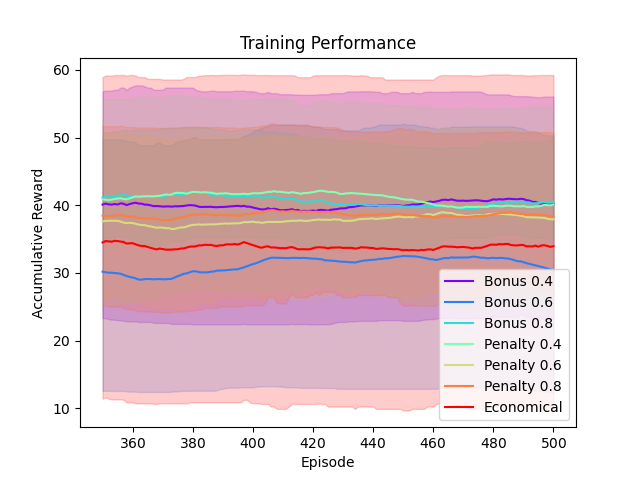
\includegraphics[width=.45\textwidth]{graphs/reward/training_performance.png}}
	\hskip1ex
	\subfloat{}{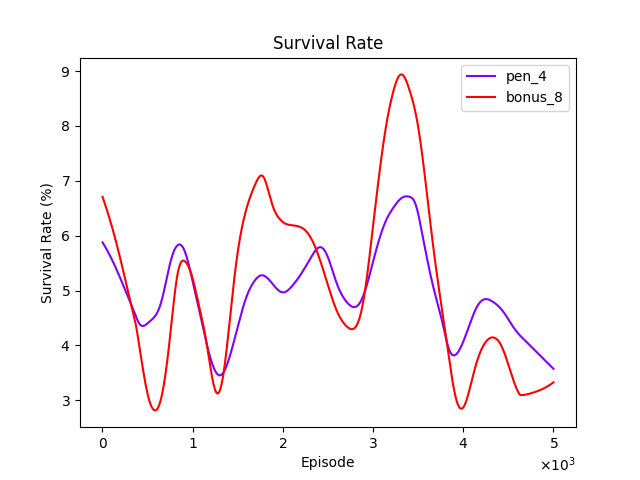
\includegraphics[width=.45\textwidth]{graphs/reward/survival_rate.png}} 
	\vfill
	\subfloat{}{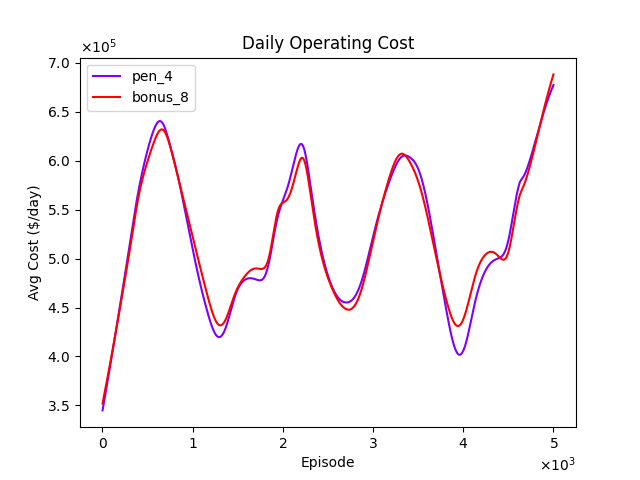
\includegraphics[width=.45\textwidth]{graphs/reward/daily_cost.png}} \hskip1ex
	\subfloat{}{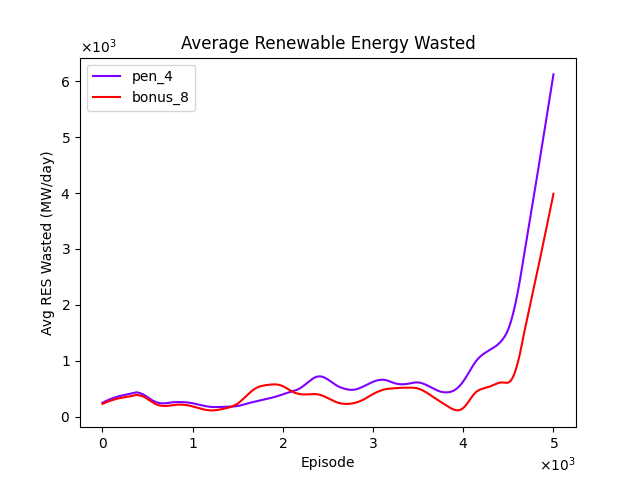
\includegraphics[width=.45\textwidth]{graphs/reward/res_wasted.png}} 
	\caption{Training Results of the best Penalty and Bonus Factor Rewards.}
	\label{fig:reward-best-train}
\end{figure}
\begin{figure}[H]
	\centering
	\subfloat{}{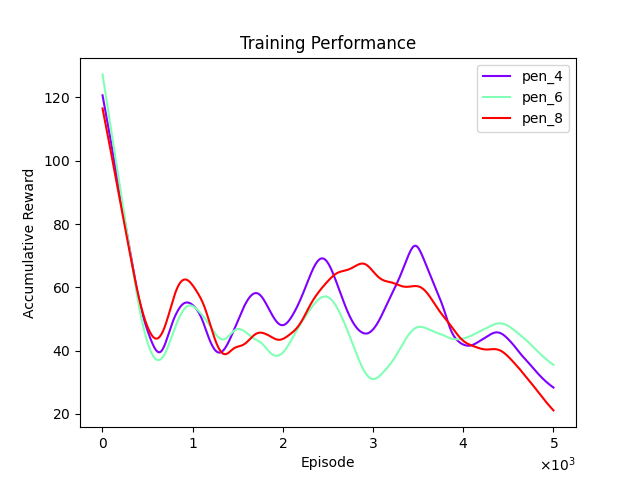
\includegraphics[width=.45\textwidth]{graphs/reward/penalty/training_performance.png}}
	\hskip1ex
	\subfloat{}{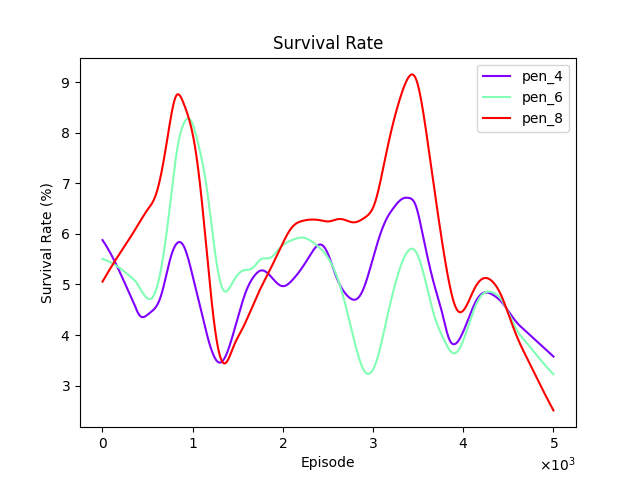
\includegraphics[width=.45\textwidth]{graphs/reward/penalty/survival_rate.png}} 
	\vfill
	\subfloat{}{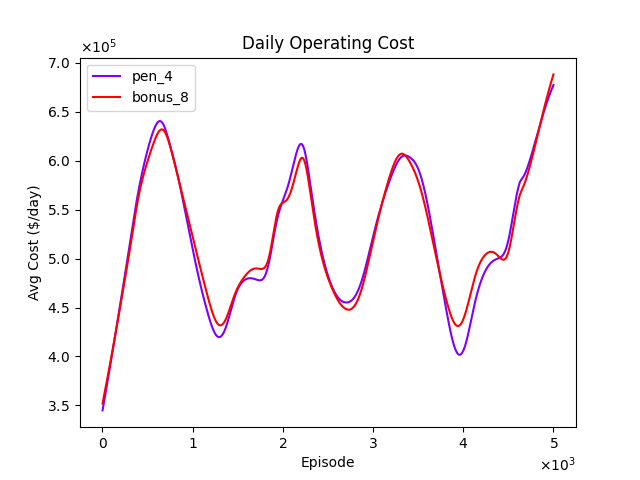
\includegraphics[width=.45\textwidth]{graphs/reward/daily_cost.png}} \hskip1ex
	\subfloat{}{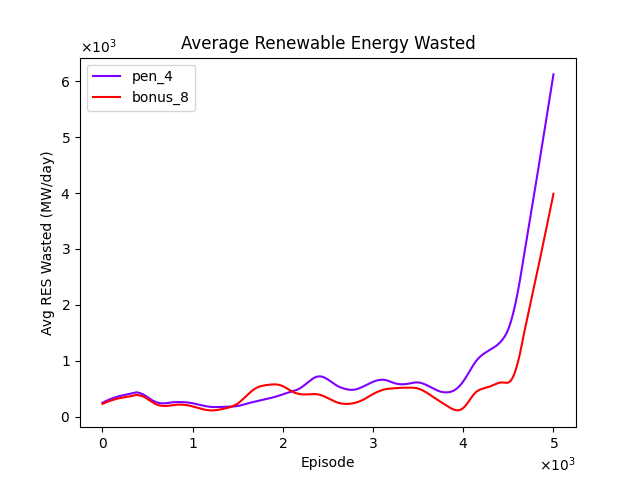
\includegraphics[width=.45\textwidth]{graphs/reward/res_wasted.png}} 
	\caption{Training Results of the Penalty Factor Rewards.}
	\label{fig:reward-pen-train}
\end{figure}

\begin{table}[ht]
	\centering
	\begin{tabularx}{\textwidth}{|l|X|X|X|X|X|}
		\hline
		\textbf{Model} & \textbf{Avg. Accumulative Reward}& \textbf{Avg. Length (Steps)} & \textbf{Avg Daily Operating Cost (€)} & \textbf{Avg. Renewables Wasted (MW/day)} & \textbf{Total Time (Seconds)}\\
		\hline
		pen\_4 & 40.57 & 80.75 & 565893.63 & 4100.20 & 230.99 \\
		pen\_6 & 37.54 & 81.40 & 558362.82 & 2570.71 & 231.09 \\
		pen\_8 & 38.22 & 76.35 & 555582.14 & 2612.34 & 222.58 \\
		bon\_4 & 40.13 & 76.23 & 565757.16 & 3723.72 & 223.90 \\
		bon\_6 & 30.78 & 55.06 & 566786.07 & 2750.34 & 189.01 \\
		bon\_8 & 40.88 & 96.43 & 560927.60 & 3115.18 & 256.59 \\
		\hline
	\end{tabularx}
	\caption{Validation Results of the Experiments concerning Limit Infeasible Curtail Actions.}
	\label{fig:curtail-val}
\end{table}


\section{Limit Infeasible Curtail Action Experiment Results}

\begin{figure}[H]
	\centering
	\subfloat{}{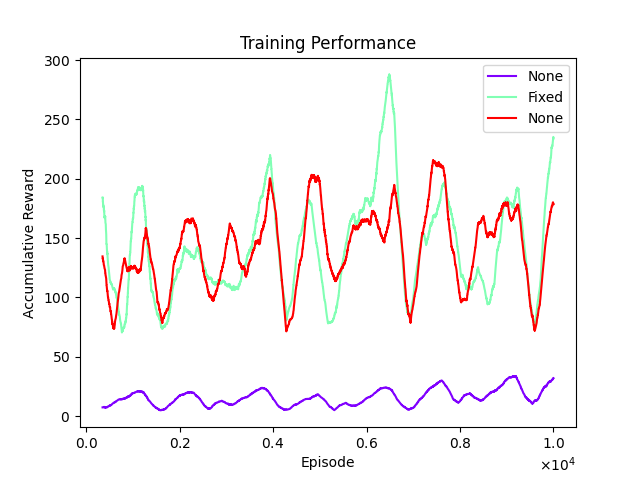
\includegraphics[width=.45\textwidth]{graphs/limit/training_performance.png}}
	\hskip1ex
	\subfloat{}{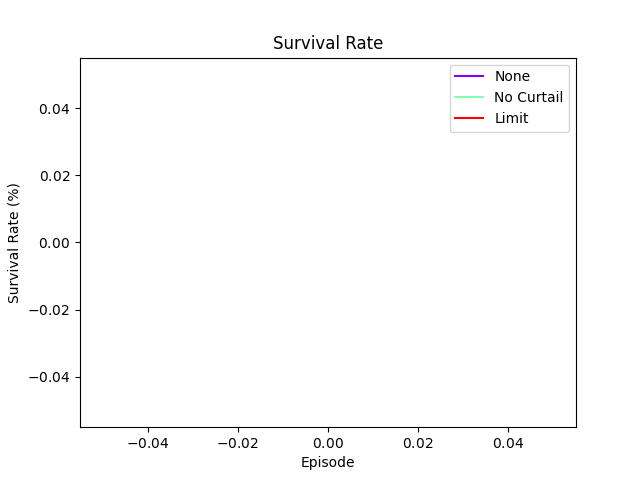
\includegraphics[width=.45\textwidth]{graphs/limit/survival_rate.png}} 
	\vfill
	\subfloat{}{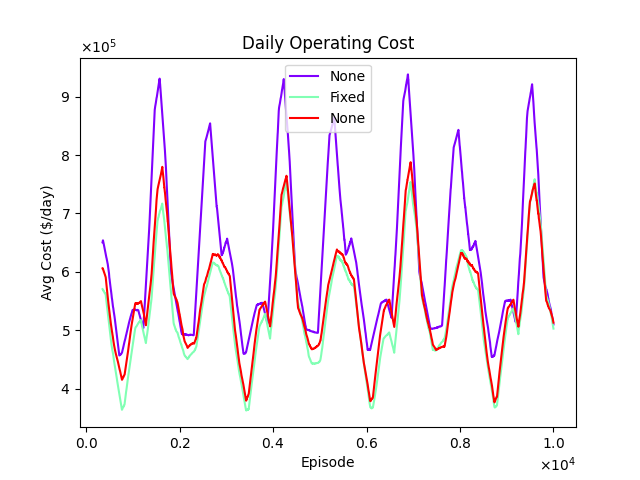
\includegraphics[width=.45\textwidth]{graphs/limit/daily_cost.png}} \hskip1ex
	\subfloat{}{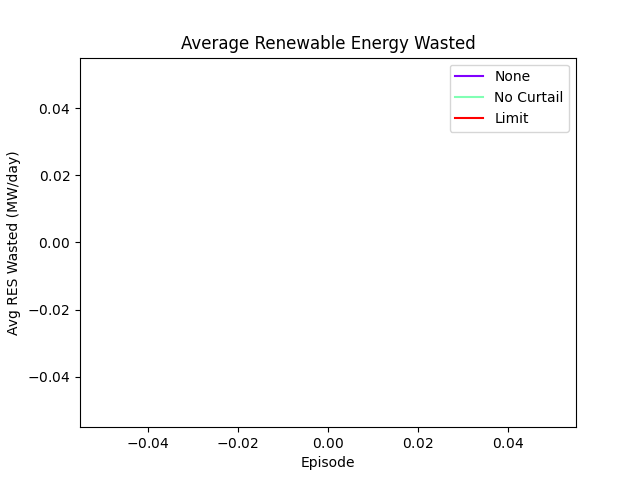
\includegraphics[width=.45\textwidth]{graphs/limit/res_wasted.png}} 
	\caption{Training Results of the Experiments concerning Limit Infeasible Curtail Actions.}
	\label{fig:curtail-train}
\end{figure}

\begin{table}[ht]
	\centering
	\begin{tabularx}{\textwidth}{|l|X|X|X|X|X|}
		\hline
		\textbf{Model} & \textbf{Avg. Accumulative Reward}& \textbf{Avg. Length (Steps)} & \textbf{Avg Daily Operating Cost (€)} & \textbf{Avg. Renewables Wasted (MW/day)} & \textbf{Total Time (Seconds)}\\
		\hline
		no\_curtail & 133.564 & 515.807  & 531470.223 & 0.0 & 692.832\\
		no\_limit & 128.173 & 403.515 & 585853.240 & 6564.428 & 569.376 \\
		limit\_curtail & 127.951 &  492.732 & 572004.947 & 8877.733 & 678.717 \\
		\hline
	\end{tabularx}
	\caption{Validation Results of the Experiments concerning Limit Infeasible Curtail Actions.}
	\label{fig:curtail-val}
\end{table}

\section{Curtailment Lower Limit Smoothing}

\begin{figure}[H]
	\centering
	\subfloat{}{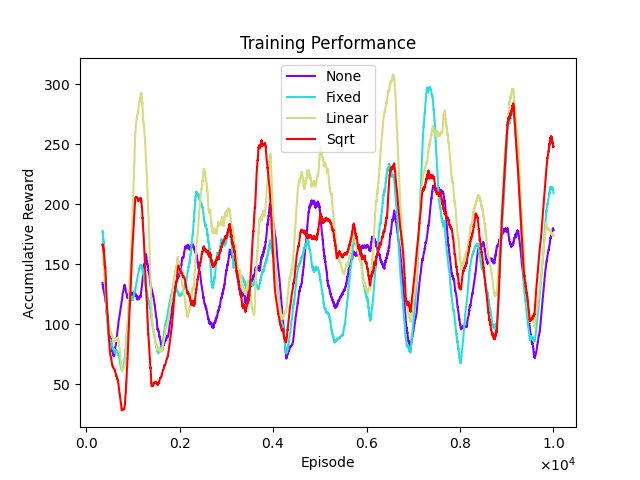
\includegraphics[width=.45\textwidth]{graphs/lower/training_performance.png}}
	\hskip1ex
	\subfloat{}{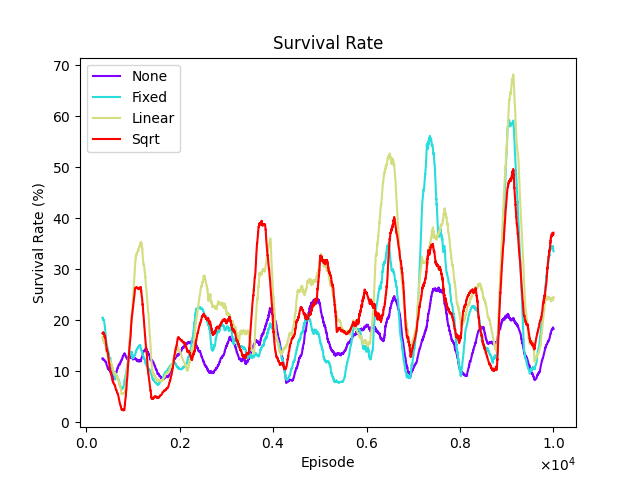
\includegraphics[width=.45\textwidth]{graphs/lower/survival_rate.png}} 
	\vfill
	\subfloat{}{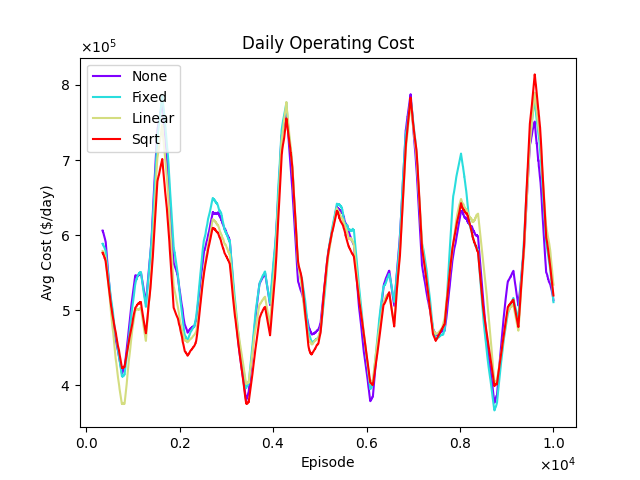
\includegraphics[width=.45\textwidth]{graphs/lower/daily_cost.png}} \hskip1ex
	\subfloat{}{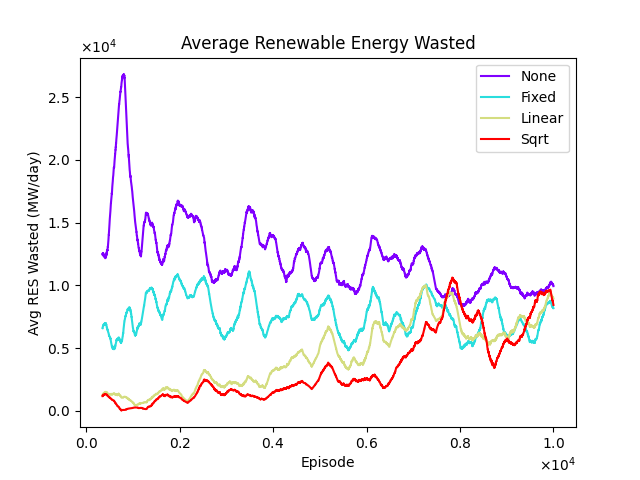
\includegraphics[width=.45\textwidth]{graphs/lower/res_wasted.png}} 
	\caption{Training Results of the Experiments concerning Curtailment Lower Limit Smoothing.}
	\label{fig:curtail-smooth-train}
\end{figure}

\begin{table}[ht]
	\centering
	\begin{tabularx}{\textwidth}{|l|X|X|X|X|X|}
		\hline
		\textbf{Model} & \textbf{Avg. Accumulative Reward}& \textbf{Avg. Length (Steps)} & \textbf{Avg Daily Operating Cost (€)} & \textbf{Avg. Renewables Wasted (MW/day)} & \textbf{Total Time (Seconds)}\\
		\hline
		none & 111.495 & 544.295 & 577960.425 & 12111.066 & 730.146 \\
		fixed & 185.698 & 761.281 & 574382.241 & 7081.859 & 1007.278 \\
		linear & 176.919 & 806.186 & 569758.273 & 5400.686 & 1052.257 \\
		sqrt & 127.951 &  492.732 & 572004.947 & 8877.733 & 678.717 \\
		\hline
	\end{tabularx}
	\caption{Validation Results of the Experiments concerning Limit Infeasible Curtail Actions.}
	\label{fig:curtail-val}
\end{table}

\begin{figure}[H]
	\centering
	\subfloat{}{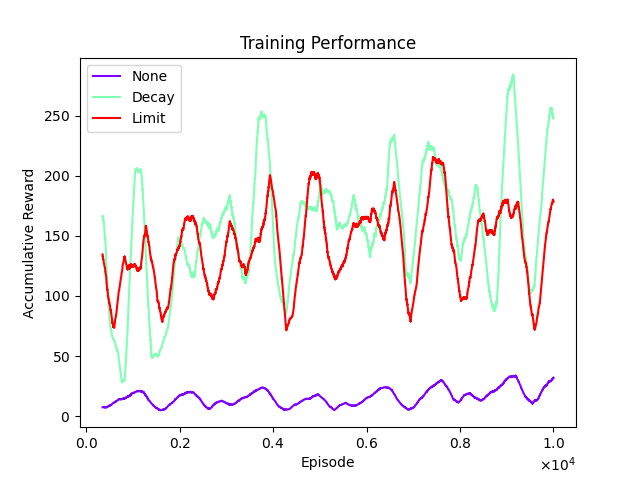
\includegraphics[width=.45\textwidth]{graphs/curtail_method/training_performance.png}}
	\hskip1ex
	\subfloat{}{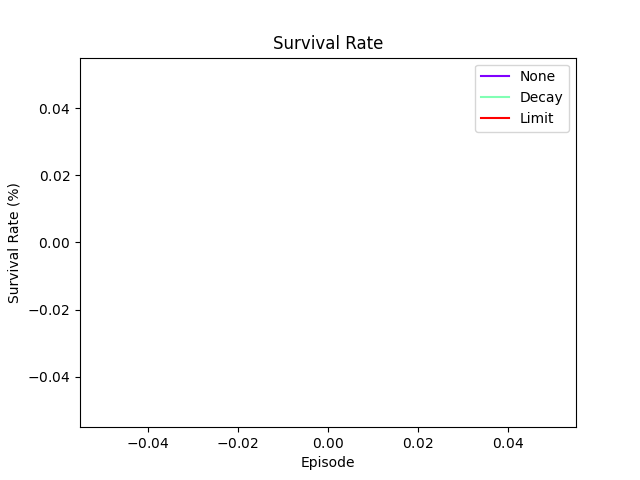
\includegraphics[width=.45\textwidth]{graphs/curtail_method/survival_rate.png}} 
	\vfill
	\subfloat{}{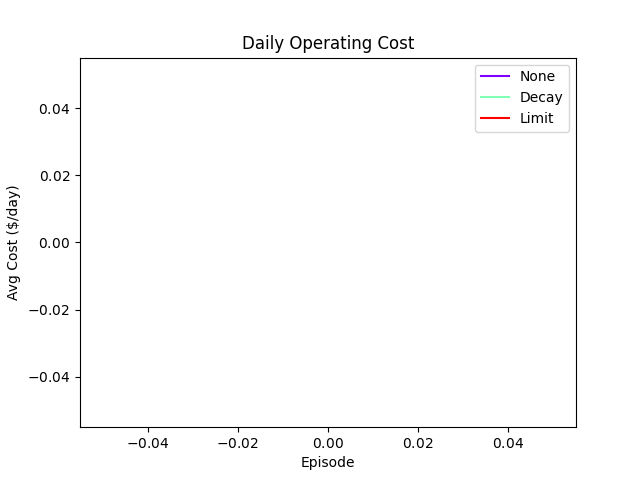
\includegraphics[width=.45\textwidth]{graphs/curtail_method/daily_cost.png}} \hskip1ex
	\subfloat{}{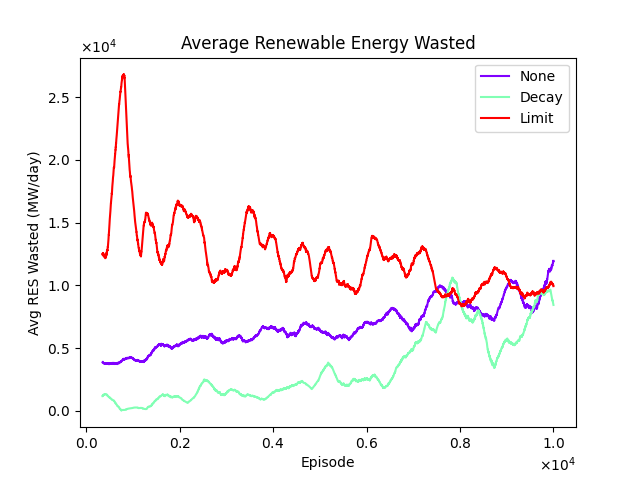
\includegraphics[width=.45\textwidth]{graphs/curtail_method/res_wasted.png}} 
	\caption{Training Results of the Experiments concerning Curtailment Lower Limit Smoothing.}
	\label{fig:curtail-smooth-train}
\end{figure}


\section{Experiments on the \ac{GNN} Tuning}

\begin{table}
	\begin{tabular}{|l|l|}
		\hline
		\textbf{Parameter} & \textbf{Values} \\
		\hline
		Aggregation Function & \{'sum','mean', 'min', 'max', 'mul'\} \\
		\hline
		Number of Layers & \{1,2,3,4,5\} \\
		\hline
		Hidden Channels & \{6, 12, 18, 24, 36\} \\
		\hline
		Ouput Channels & \{3, 6, 12, 18, 24, 36\} \\
		\hline 
		Dropout Rate & [0.1, 0.4] \\
		\hline
		Activation First & {True, False} \\
		\hline 
		Heads & {1,2,3,6} \\
		\hline
		GATv2 & {True, False} \\
		\hline
	\end{tabular}
	\caption{General \ac{GNN} Parameters Tuned}
\end{table}

\begin{table}
	\begin{tabular}{|l|l|l|}
		\hline
		\textbf{Implementation} & \textbf{Parameter} & \textbf{Values} \\
		\hline
		GCN & Improved & {True, False} \\
		\hline 
		GAT & Heads & {1,2,3,6} \\
		\hline
		GAT & GATv2 & {True, False} \\
		\hline
	\end{tabular}
	\caption{Model-Specific Parameters Tuned}
\end{table}



\section{Experiments on the \ac{GCN} Aggregation Function} \label{appendix:aggr}

\begin{table}
	\begin{tabular}{|l|l|}
		\hline
		\textbf{Parameter} & \textbf{Values} \\
		\hline
		Aggregation Function & \{'sum','mean', 'min', 'max', 'mul'\} \\
		\hline
		Number of Layers & 1 \\
		\hline
		Hidden Channels & 18 \\
		\hline
		Ouput Channels & 6 \\
		\hline 
		Dropout Rate & 0.1 \\
		\hline
		Activation First & True \\
		\hline
	\end{tabular}
	\caption{Parameters of Aggregation Function Experiment}
	\label{table:aggr-params}
\end{table}

\begin{figure}[H]
	\centering
	\subfloat{}{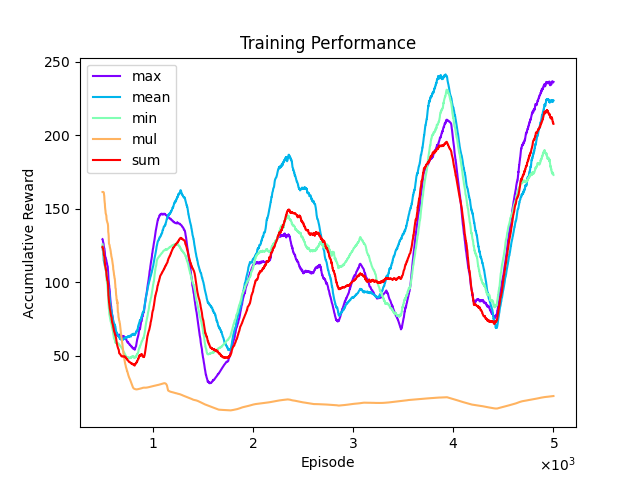
\includegraphics[width=.45\textwidth]{graphs/aggr/training_performance.png}}
	\hskip1ex
	\subfloat{}{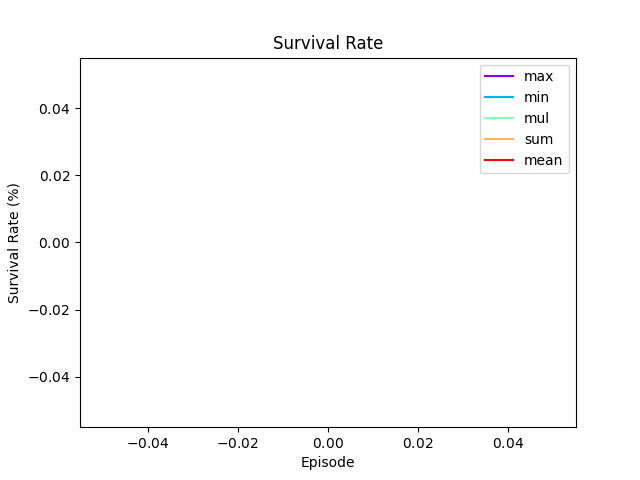
\includegraphics[width=.45\textwidth]{graphs/aggr/survival_rate.png}} 
	\vfill
	\subfloat{}{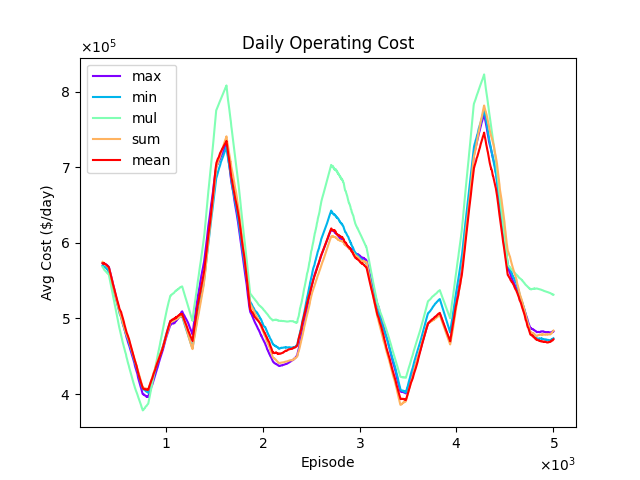
\includegraphics[width=.45\textwidth]{graphs/aggr/daily_cost.png}} \hskip1ex
	\subfloat{}{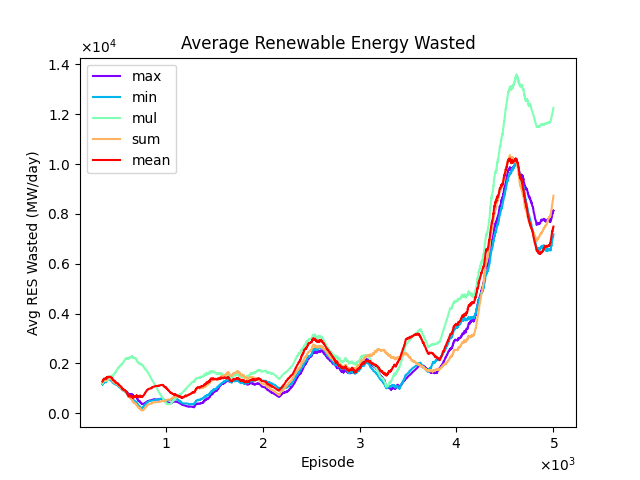
\includegraphics[width=.45\textwidth]{graphs/aggr/res_wasted.png}} 
	\caption{Training Results of different types of \ac{GNN} aggregation functions}
	\label{fig:aggr-train}
\end{figure}

	\begin{table}[ht]
		\centering
		\begin{tabularx}{\textwidth}{|l|X|X|X|X|X|}
			\hline
			\textbf{Model} & \textbf{Avg. Accumulative Reward}& \textbf{Avg. Length (Steps)} & \textbf{Avg Daily Operating Cost (€)} & \textbf{Avg. Renewables Wasted (MW/day)} & \textbf{Total Time (Seconds)}\\
			\hline
			max & 119.16 & 677.75 & 560219.45 & 6564.49 & 552.51\\
			sum & 114.58 & 768.58 & 569952.37 & 7268.28 &  606.28 \\
			mean & 92.90 &  551.24 & 557637.84 & 6268.06 & 454.24 \\
			min & 80.89 & 495.70 & 559033.63 & 6687.94 & 416.63 \\
			mul & 15.76 & 1104.06 & 608319.66 & 10305.96 & 846.43 \\
			\hline
		\end{tabularx}
		\caption{Validation Results of different types of \ac{GNN} aggregation functions.}
		\label{table:aggr-val}
	\end{table}

\section{Experiments on the number of \ac{GCN} layers}

\begin{table}
	\begin{tabular}{|l|l|}
		\hline
		\textbf{Parameter} & \textbf{Values} \\
		\hline
		Aggregation Function & 'max' \\
		\hline
		Number of Layers & [1, 6] \\
		\hline
		Hidden Channels & 18 \\
		\hline
		Ouput Channels & 6 \\
		\hline 
		Dropout Rate & 0.1 \\
		\hline
		Activation First & True \\
		\hline 
		\hline
	\end{tabular}
	\caption{General \ac{GNN} Parameters Tuned}
\end{table}

\begin{figure}[H]
	\centering
	\subfloat{}{\includegraphics[width=.45\textwidth]{graphs/layers/training_performance.png}}
	\hskip1ex
	\subfloat{}{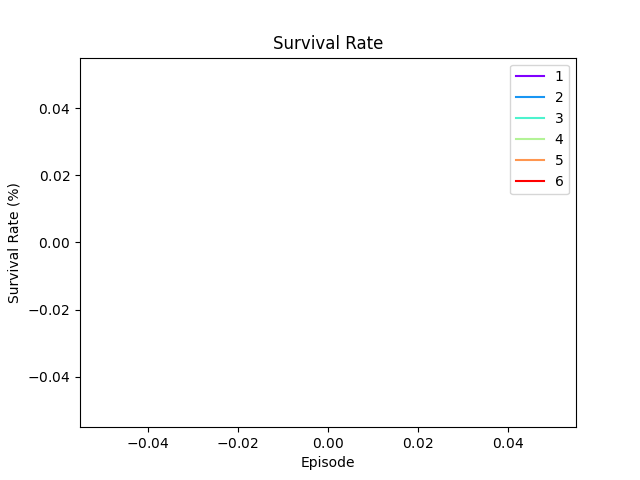
\includegraphics[width=.45\textwidth]{graphs/layers/survival_rate.png}} 
	\vfill
	\subfloat{}{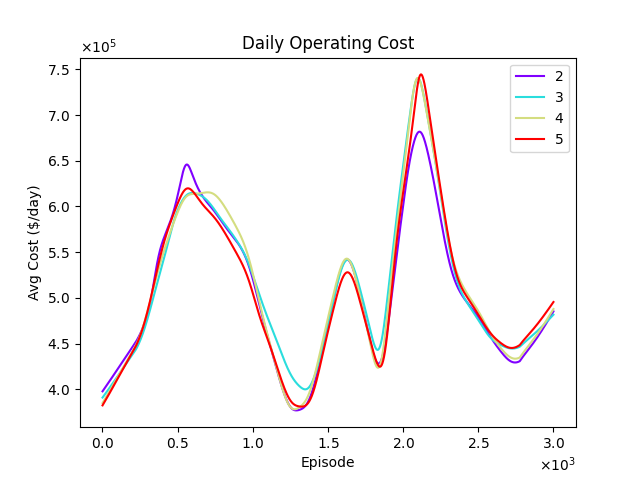
\includegraphics[width=.45\textwidth]{graphs/layers/daily_cost.png}} \hskip1ex
	\subfloat{}{\includegraphics[width=.45\textwidth]{graphs/layers/res_wasted.png}} 
	\caption{Training Results of models with 2, 3, 4 and 5 \ac{GNN} Layers}
	\label{fig:gnn-layers-train}
\end{figure}


\begin{table}[ht]
	\centering
	\begin{tabularx}{\textwidth}{|l|X|X|X|X|X|}
		\hline
		\textbf{Model} & \textbf{Avg. Accumulative Reward}& \textbf{Avg. Length (Steps)} & \textbf{Avg Daily Operating Cost (€)} & \textbf{Avg. Renewables Wasted (MW/day)} & \textbf{Total Time (Seconds)}\\
		\hline
		6 & 135.75 & 487.09 & 560147.77 & 5862.49 & 655.44 \\
		3 & 110.73 & 736.32 & 567510.58 & 7116.24 & 744.50 \\
		1 & 101.24 & 709.76 & 565865.82 & 6855.58 & 573.30 \\
		4 & 98.67 & 451.51 & 577464.90 & 8641.05 & 529.76 \\
		5 & 92.97 & 286.65 & 550205.21 & 6397.41 & 386.19 \\
		2 & 91.58 & 694.67 & 575093.64 & 5989.95 & 638.11 \\
		\hline
	\end{tabularx}
	\caption{Validation Results of the Experiments concerning Limit Infeasible Curtail Actions.}
	\label{fig:curtail-val}
\end{table}

\section{Experiments on the \ac{GNN} Parameters \textit{act\_first} and \textit{improved}}

\begin{figure}[H]
	\centering
	\subfloat{}{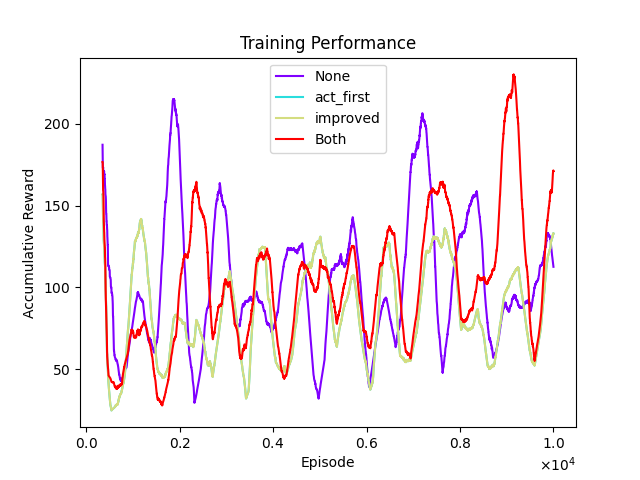
\includegraphics[width=.45\textwidth]{graphs/gcn_param/training_performance.png}}
	\hskip1ex
	\subfloat{}{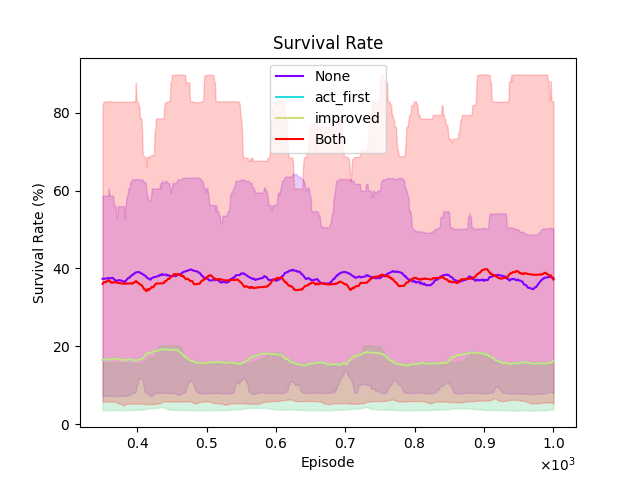
\includegraphics[width=.45\textwidth]{graphs/gcn_param/survival_rate.png}} 
	\vfill
	\subfloat{}{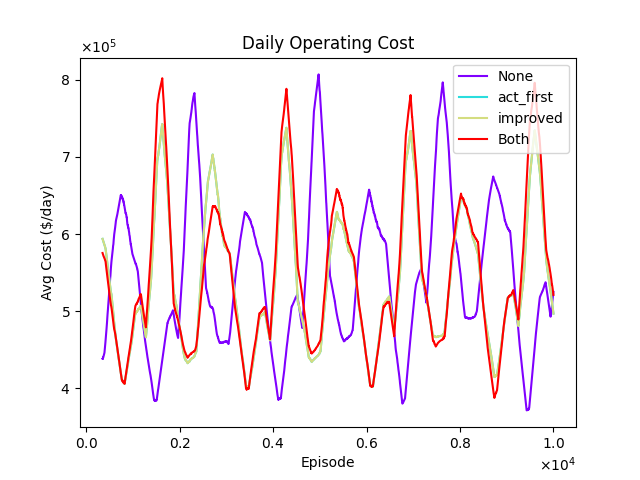
\includegraphics[width=.45\textwidth]{graphs/gcn_param/daily_cost.png}} \hskip1ex
	\subfloat{}{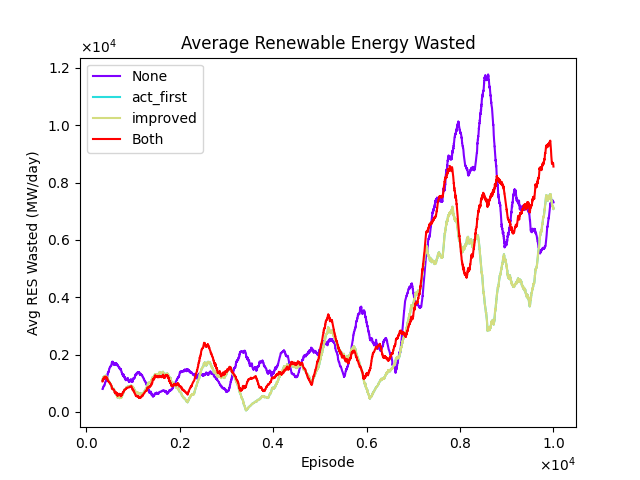
\includegraphics[width=.45\textwidth]{graphs/gcn_param/res_wasted.png}} 
	\caption{Training Results of the act\_first and improved Parameter Tests.}
	\label{fig:act-first-improved-train}
\end{figure}

\begin{comment}
	\begin{table}[ht]
		\centering
		\begin{tabularx}{\textwidth}{|l|X|X|X|X|X|}
			\hline
			\textbf{Model} & \textbf{Avg. Accumulative Reward}& \textbf{Avg. Length (Steps)} & \textbf{Avg Daily Operating Cost (€)} & \textbf{Avg. Renewables Wasted (MW/day)} & \textbf{Total Time (Seconds)}\\
			\hline
			none & & & & & \\
			act\_first & & & & & \\
			improved & & & & & \\
			act\_first\_improved & & & & &  \\
			\hline
		\end{tabularx}
		\caption{Validation Results of the Experiments concerning Limit Infeasible Curtail Actions.}
		\label{fig:curtail-val}
	\end{table}
\end{comment}

\section{Experiments on the number of \ac{GAT} Heads}

\begin{figure}[H]
	\centering
	\subfloat{}{\includegraphics[width=.45\textwidth]{graphs/gat_param/training_performance.png}}
	\hskip1ex
	\subfloat{}{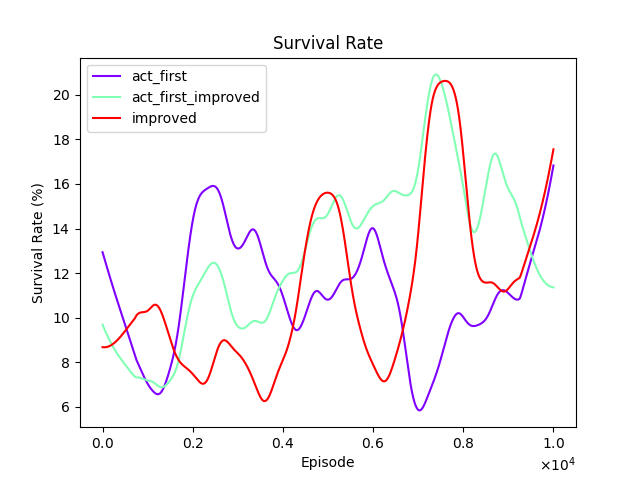
\includegraphics[width=.45\textwidth]{graphs/gat_param/survival_rate.png}} 
	\vfill
	\subfloat{}{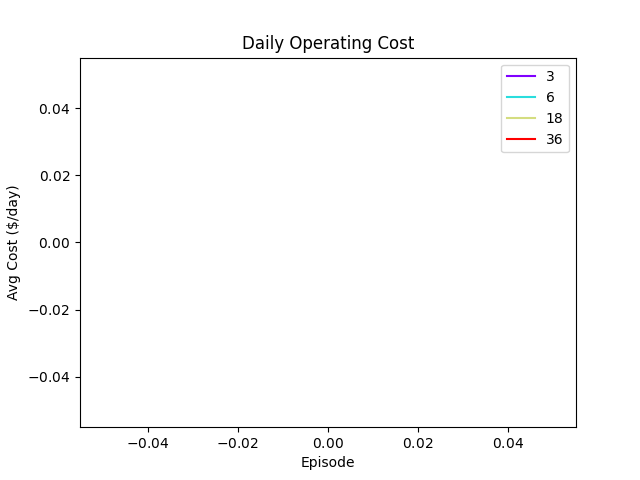
\includegraphics[width=.45\textwidth]{graphs/gat_param/daily_cost.png}} \hskip1ex
	\subfloat{}{\includegraphics[width=.45\textwidth]{graphs/gat_param/res_wasted.png}} 
	\caption{Training Results of models with 1, 2 and 3 \ac{GAT} Heads}
	\label{fig:gat-heads-train}
\end{figure}

\begin{comment}
\begin{table}[ht]
	\centering
	\begin{tabularx}{\textwidth}{|l|X|X|X|X|X|}
		\hline
		\textbf{Model} & \textbf{Avg. Accumulative Reward}& \textbf{Avg. Length (Steps)} & \textbf{Avg Daily Operating Cost (€)} & \textbf{Avg. Renewables Wasted (MW/day)} & \textbf{Total Time (Seconds)}\\
		\hline
		1 & & & & & \\
		2 & & & & & \\
		3 & & & & & \\
		\hline
	\end{tabularx}
	\caption{Validation Results of the Experiments concerning Limit Infeasible Curtail Actions.}
	\label{fig:curtail-val}
\end{table}
\end{comment}

\section{GNNs vs. SAC Experiments}

\begin{figure}[H]
	\centering
	\subfloat{}{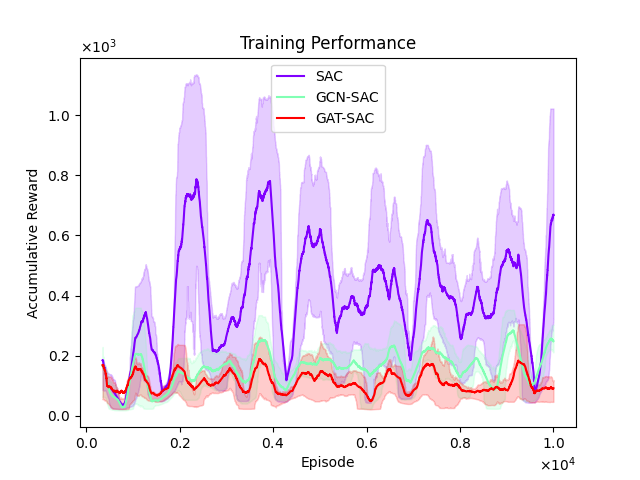
\includegraphics[width=.45\textwidth]{graphs/36/training_performance.png}}
	\hskip1ex
	\subfloat{}{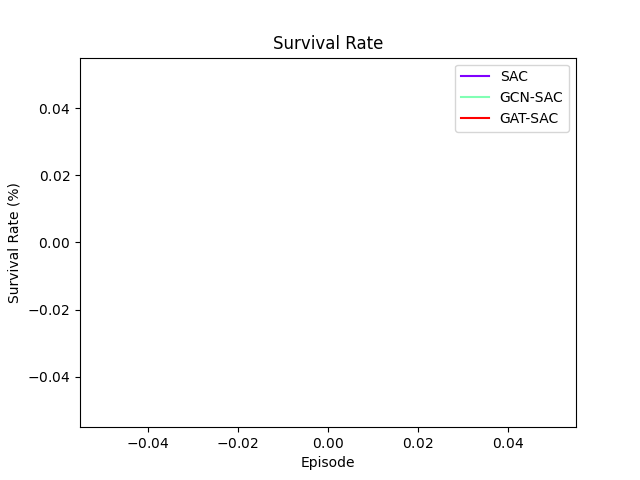
\includegraphics[width=.45\textwidth]{graphs/36/survival_rate.png}} 
	\vfill
	\subfloat{}{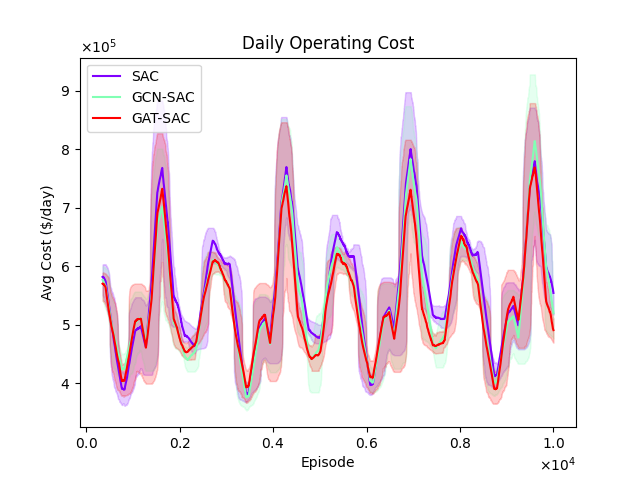
\includegraphics[width=.45\textwidth]{graphs/36/daily_cost.png}} \hskip1ex
	\subfloat{}{\includegraphics[width=.45\textwidth]{graphs/36/res_wasted.png}} 
	\caption{Training Results of models with 1, 2 and 3 \ac{GAT} Heads}
	\label{fig:gnns-train}
\end{figure}

	\begin{table}[ht]
		\centering
		\begin{tabularx}{\textwidth}{|l|X|X|X|X|X|}
			\hline
			\textbf{Model} & \textbf{Avg. Accumulative Reward}& \textbf{Avg. Length (Steps)} & \textbf{Avg Daily Operating Cost (€)} & \textbf{Avg. Renewables Wasted (MW/day)} & \textbf{Total Time (Seconds)}\\
			\hline
			sac & 342.84 & 1118.24 & 601896.44 & 5443.64 & 741.23 \\
			gcn\_sac & 23.38 & 573.73 & 549592.13 & 9885.84 & 467.29 \\
			gat\_sac & 55.80 & 481.72  & 553388.36 & 6064.43 & 603.91 \\
			\hline
		\end{tabularx}
		\caption{Validation Results of the Experiments concerning Limit Infeasible Curtail Actions.}
		\label{fig:curtail-val}
	\end{table}



\section{Experiments on 118-bus scenario}

\begin{figure}[H]
	\centering
	\subfloat{}{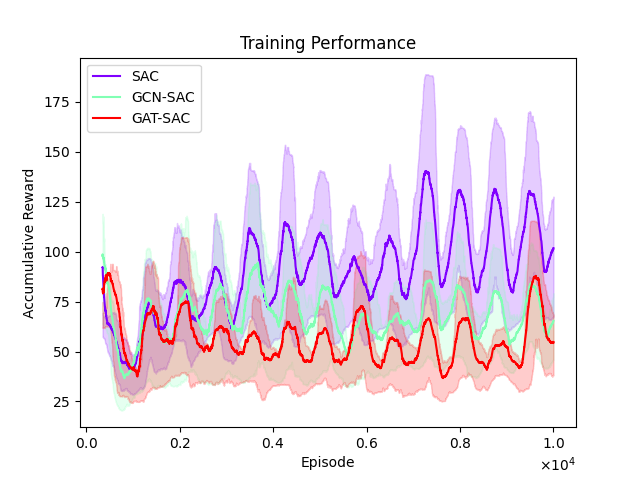
\includegraphics[width=.45\textwidth]{graphs/118/training_performance.png}}
	\hskip1ex
	\subfloat{}{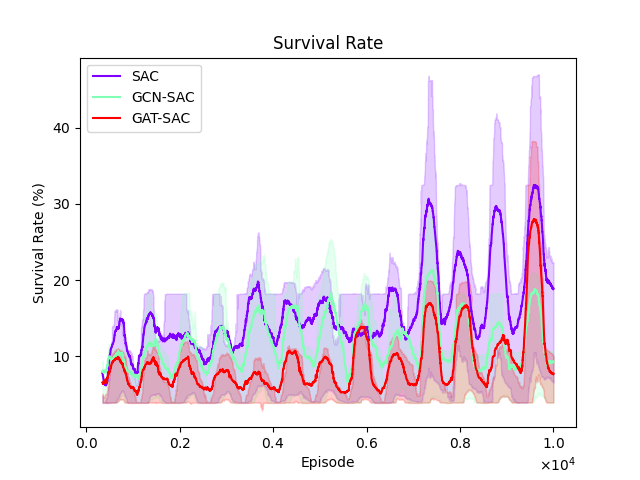
\includegraphics[width=.45\textwidth]{graphs/118/survival_rate.png}} 
	\vfill
	\subfloat{}{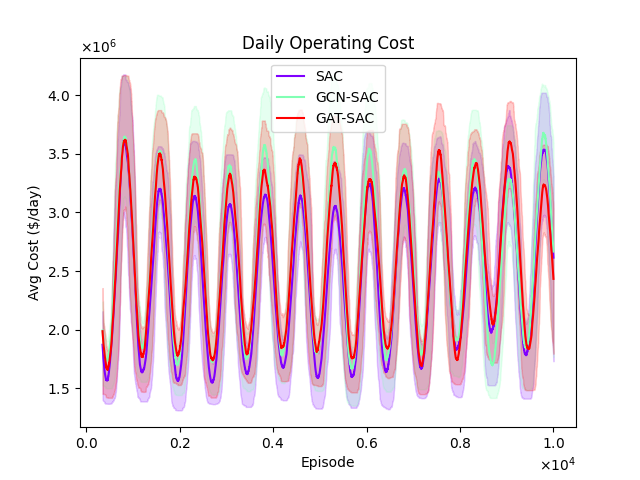
\includegraphics[width=.45\textwidth]{graphs/118/daily_cost.png}} \hskip1ex
	\subfloat{}{\includegraphics[width=.45\textwidth]{graphs/118/res_wasted.png}} 
	\caption{Training Results of models with 1, 2 and 3 \ac{GAT} Heads}
	\label{fig:118-train}
\end{figure}


	\begin{table}[ht]
		\centering
		\begin{tabularx}{\textwidth}{|l|X|X|X|X|X|}
			\hline
			\textbf{Model} & \textbf{Avg. Accumulative Reward}& \textbf{Avg. Length (Steps)} & \textbf{Avg Daily Operating Cost (€)} & \textbf{Avg. Renewables Wasted (MW/day)} & \textbf{Total Time (Seconds)}\\
			\hline
			sac & 342.838 & 1118.241 & 601896.445 & 5443.649 & 756.142 \\
			gcn\_sac & 11.74 & 815.64 & 2679050.39 & 6567.22 & 318.94 \\
			\hline
		\end{tabularx}
		\caption{Validation Results of the Experiments concerning Limit Infeasible Curtail Actions.}
		\label{fig:curtail-val}
	\end{table}
	